\documentclass[../main.tex]{subfiles}

\begin{document}
	\section{Grundlagen}
	
	\subsection{Hosting}
	Unser Produkt soll auf dem neusten Stand der Dinge sein und daher verzichten wir auf den Hoster Hosttech der schon für das bestehende System verwendet wird. Ein grosser Nachteil von Hosttech ist das wir auf ein PHP Backend beschränkt sind. Um auch das Deployment zu modernisieren und hauptsächlich zu automatisieren möchten wir mit Dockercontainer arbeiten. Hierbei hat unser Betreuer seine Plattform angeboten. Auf dieser können wir ein Image des Dockercontainers hosten lassen. Somit ist dieses zu jederzeit erreichbar. Dies gilt für das Frontend sowie für das Backend.
	Damit der Server nach der Umsetzung nach wie vor erreichbar ist, wurde uns vom Betreuer folgende Seite vorgeschlagen: https://www.hetzner.com/de/
	
	\subsection{Backend Technologie}
	Mit dem Loslösen von Hosttech sind wir frei die Backend Technologie zu bestimmen und wir haben uns auf Java/Spring-Boot geeinigt. Wir haben uns für Spring-Boot entschieden, da alle Entwickler mit Java vertraut sind und OpenAPI Spring-Boot unterstützt. Spring-Boot eignet sich auch gut für unsere Aufgabenstellung, da wir eine Datenbank anschliessen werden und die Daten auf der Webseite nicht nur dargestellt werden sondern auch manipuliert werden können, eignet sich Spring-Boot mit der einfachen Handhabung von JPA gut.
	
	\subsection{Schnittstelle}
	Als Schnittstelle zwischen Backend und Frontend wollen wir das State of the Art Tool OpenAPI einsetzen. Nach genauerer Analyse sehen wir einen grossen Nutzen des Tools, da es uns eine grosse Unterstützung zur Entwicklung der REST Schnittstelle sein wird. In OpenAPI kann in einem YAML File die ganze REST Schnittstelle erstellt und konfiguriert werden daraus kann dann OpenAPI unser Spring-Boot Backend erzeugen was uns viel Arbeit abnimmt.
	
	\subsection{Frontend Technologie}
	Als Frontend-Framework sind wir frei, da es keinen Wunsch/Voraussetzung vom Kunden gab.
	Wir als Gruppe haben uns für Angular(2+) aus mehreren Gründen entschieden. \\
	\\
	Zum Einen kennt sich die Merhheit der Gruppe gut mit dem Framework aus, dadurch fällt der Einstieg etwas leichter. Zum Anderen ist die Verwendung von guten Templates einfach und effizient. Die Benutzung von einem Template und Komponenten, welche übersichtlich und flexibel verwendet werden können, war für uns ein ausschlaggebender Punkt. \\ 
	Aus diesen Gründen kam Angular für uns an 1. Stelle zur Sprache
	
	
	\subsection{Datenbank}
	Um den alten Stand weiterzuführen, wird weiterhin die mySQL Datenbank benutzt. Diese wird mithilfe der Schnittstelle angepasst.
	Die bestehende Datenbank auf Hosttech wird in einen neuen Docker-Container migriert und neben dem Spring-Boot Projekt gehostet. Nur das Spring-Boot Projekt hat direkten Zugriff auf die Datenbank, alle Änderungen müssen über die REST Schnittstelle der Spring-Boot Applikation erfolgen.
	
	\begin{figure}[H]
		\centering
		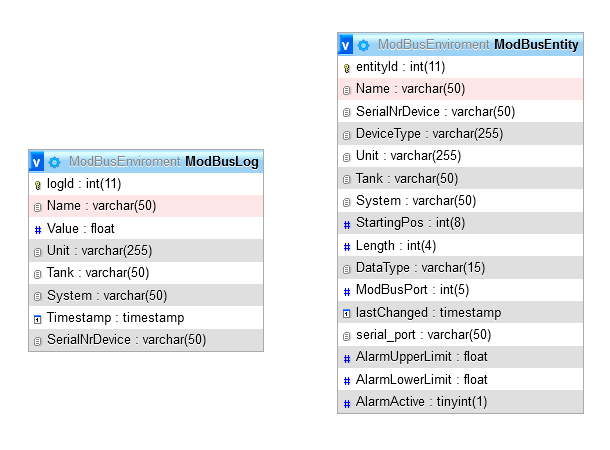
\includegraphics[scale=0.8]{datenbank_overview}
		\caption{Datenbank Überblick}
		\label{fig:datenbank_overview}
	\end{figure}
	
	Nach Analyse der Datenbank sahen wir ebenfalls Potential für Verbesserungen, doch wollten wir nicht zu viel an der Struktur ändern, da diese Änderungen weitere Anpassungen auf Systemen erfordern, welche wir keinen Einfluss nehmen können, daher haben wir uns entschieden die Datenbank zu belassen und eine 1 zu 1 Kopie zu erstellen.
\end{document}